\section{Plagiarism Detection}

\subsection{Introduction}
Plagiarism detection in code is the method and process used for locating instances of cloned code within a set of documents. The tool we have chosen to demonstrate and explore plagiarism detection is JPlag. 

\subsection{JPlag}
JPlag is a system that finds similarities, software plagiarisms, among multiple source code files. It is robust against many attempts to disguise the copied code because it is aware of programming language syntax and program structure. Thus, it is very hard to deceive: 90\% of plagiarisms are detected and the rest raise suspicion. [4] Moreover, JPlag is able to process a hundred programs with several hundred lines of code in seconds, making it a very robust and scalable tool. 
It has been successfully used for detecting plagiarism among students’ Java programs but support for other languages such as C and C++ are also available.\\\\
JPlag’s comparison algorithm is based on the “Greedy String Tiling” [5], which takes in a set of program source code as input and outputs a similarity score between pairs of programs and their corresponding similarity regions. To do so, it must initially convert the program source code in to token strings, this is the only language dependent process involve din JPlag’s plagiarism detection. Tokens should be chosen in a manner, which captures the essence of the program’s structure rather than the surface aspects, as a program’s structure is harder for plagiarists to modify. JPlag does this phase whilst ignoring whitespaces, comments and names of identifiers. Figure \ref{fig:sample} shows an example Java code and its corresponding tokens generated by JPlag. A list of possible JPlag tokens can be found in this technical report [6].\\\\
\begin{figure} [ht]
\centering
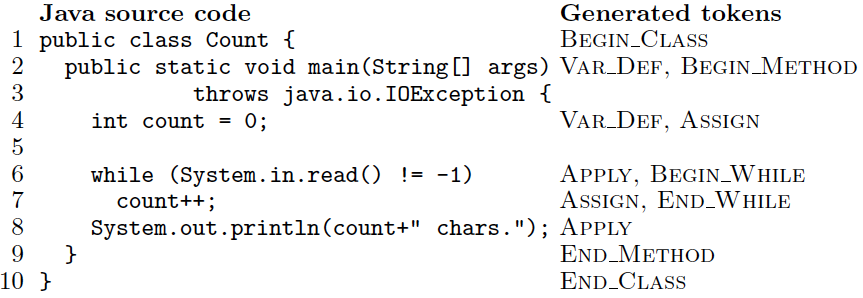
\includegraphics[width=0.7\textwidth]{Figures/samplecode}
\caption{A sample Java Source code with the generated token strings}
\label{fig:sample}
\end{figure}
Once the token strings have been generated, JPlag beings the comparison phase by comparing the two generated token strings. When comparing two strings A and B, JPlag’s objective is to discover a maximal set of contiguous substrings. Each substring must occur in both A and B and must be as long as possible. These substrings (matches) must be unique in that each substring should not cover tokens already covered by other substrings. To avoid false matches, a minimum match length M is enforced. 

\subsection{Greedy Tiling Algorithm}
The Greedy String Tiling algorithm itself has two steps shown in Figure \ref{fig:greedy}. Firstly, all substrings common to both token strings are found with lengths equal to or greater than the minimum M. Secondly, all the tokens found in the substrings are marked so that they are no longer picked up by subsequent iterations of the first step. By marking its tokens, a match becomes a “tile”. Thus, the similarity score between is calculated based on the fraction of tokens that were found as matches:

\begin{equation}
    sim(A,B) = \frac{2 * coverage(tiles)}{|A|+|B|}
\end{equation}
\begin{figure} [ht]
\centering
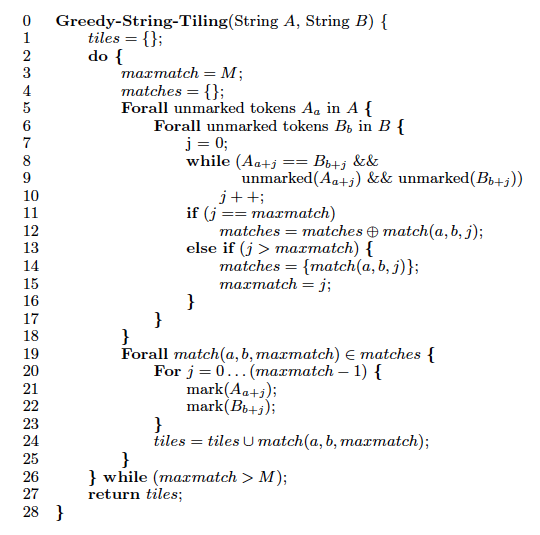
\includegraphics[width=0.7\textwidth]{Figures/stringtiling}
\caption{Greedy String Tiling algorithm}
\label{fig:greedy}
\end{figure}

\break